% Options for packages loaded elsewhere
\PassOptionsToPackage{unicode}{hyperref}
\PassOptionsToPackage{hyphens}{url}
%
\documentclass[
]{article}
\usepackage{amsmath,amssymb}
\usepackage{lmodern}
\usepackage{setspace} % add line to default template
\setstretch{1.2}      % add line to default template
\usepackage{iftex}
\ifPDFTeX
  \usepackage[T1]{fontenc}
  \usepackage[utf8]{inputenc}
  \usepackage{textcomp} % provide euro and other symbols
\else % if luatex or xetex
  \usepackage{unicode-math}
  \defaultfontfeatures{Scale=MatchLowercase}
  \defaultfontfeatures[\rmfamily]{Ligatures=TeX,Scale=1}
\fi
% Use upquote if available, for straight quotes in verbatim environments
\IfFileExists{upquote.sty}{\usepackage{upquote}}{}
\IfFileExists{microtype.sty}{% use microtype if available
  \usepackage[]{microtype}
  \UseMicrotypeSet[protrusion]{basicmath} % disable protrusion for tt fonts
}{}
\makeatletter
\@ifundefined{KOMAClassName}{% if non-KOMA class
  \IfFileExists{parskip.sty}{%
    \usepackage{parskip}
  }{% else
    \setlength{\parindent}{0pt}
    \setlength{\parskip}{6pt plus 2pt minus 1pt}}
}{% if KOMA class
  \KOMAoptions{parskip=half}}
\makeatother
\usepackage{xcolor}
\IfFileExists{xurl.sty}{\usepackage{xurl}}{} % add URL line breaks if available
\IfFileExists{bookmark.sty}{\usepackage{bookmark}}{\usepackage{hyperref}}
\hypersetup{
  pdftitle={Statistical analysis of behavioral data},
  pdfauthor={Ahmad Ehyaei; Sara Ershadmanesh},
  hidelinks,
  pdfcreator={LaTeX via pandoc}}
\urlstyle{same} % disable monospaced font for URLs
\usepackage{color}
\usepackage{fancyvrb}
\newcommand{\VerbBar}{|}
\newcommand{\VERB}{\Verb[commandchars=\\\{\}]}
\DefineVerbatimEnvironment{Highlighting}{Verbatim}{commandchars=\\\{\}}
% Add ',fontsize=\small' for more characters per line
\usepackage{framed}
\definecolor{shadecolor}{RGB}{248,248,248}
\newenvironment{Shaded}{\begin{snugshade}}{\end{snugshade}}
\newcommand{\AlertTok}[1]{\textcolor[rgb]{0.94,0.16,0.16}{#1}}
\newcommand{\AnnotationTok}[1]{\textcolor[rgb]{0.56,0.35,0.01}{\textbf{\textit{#1}}}}
\newcommand{\AttributeTok}[1]{\textcolor[rgb]{0.77,0.63,0.00}{#1}}
\newcommand{\BaseNTok}[1]{\textcolor[rgb]{0.00,0.00,0.81}{#1}}
\newcommand{\BuiltInTok}[1]{#1}
\newcommand{\CharTok}[1]{\textcolor[rgb]{0.31,0.60,0.02}{#1}}
\newcommand{\CommentTok}[1]{\textcolor[rgb]{0.56,0.35,0.01}{\textit{#1}}}
\newcommand{\CommentVarTok}[1]{\textcolor[rgb]{0.56,0.35,0.01}{\textbf{\textit{#1}}}}
\newcommand{\ConstantTok}[1]{\textcolor[rgb]{0.00,0.00,0.00}{#1}}
\newcommand{\ControlFlowTok}[1]{\textcolor[rgb]{0.13,0.29,0.53}{\textbf{#1}}}
\newcommand{\DataTypeTok}[1]{\textcolor[rgb]{0.13,0.29,0.53}{#1}}
\newcommand{\DecValTok}[1]{\textcolor[rgb]{0.00,0.00,0.81}{#1}}
\newcommand{\DocumentationTok}[1]{\textcolor[rgb]{0.56,0.35,0.01}{\textbf{\textit{#1}}}}
\newcommand{\ErrorTok}[1]{\textcolor[rgb]{0.64,0.00,0.00}{\textbf{#1}}}
\newcommand{\ExtensionTok}[1]{#1}
\newcommand{\FloatTok}[1]{\textcolor[rgb]{0.00,0.00,0.81}{#1}}
\newcommand{\FunctionTok}[1]{\textcolor[rgb]{0.00,0.00,0.00}{#1}}
\newcommand{\ImportTok}[1]{#1}
\newcommand{\InformationTok}[1]{\textcolor[rgb]{0.56,0.35,0.01}{\textbf{\textit{#1}}}}
\newcommand{\KeywordTok}[1]{\textcolor[rgb]{0.13,0.29,0.53}{\textbf{#1}}}
\newcommand{\NormalTok}[1]{#1}
\newcommand{\OperatorTok}[1]{\textcolor[rgb]{0.81,0.36,0.00}{\textbf{#1}}}
\newcommand{\OtherTok}[1]{\textcolor[rgb]{0.56,0.35,0.01}{#1}}
\newcommand{\PreprocessorTok}[1]{\textcolor[rgb]{0.56,0.35,0.01}{\textit{#1}}}
\newcommand{\RegionMarkerTok}[1]{#1}
\newcommand{\SpecialCharTok}[1]{\textcolor[rgb]{0.00,0.00,0.00}{#1}}
\newcommand{\SpecialStringTok}[1]{\textcolor[rgb]{0.31,0.60,0.02}{#1}}
\newcommand{\StringTok}[1]{\textcolor[rgb]{0.31,0.60,0.02}{#1}}
\newcommand{\VariableTok}[1]{\textcolor[rgb]{0.00,0.00,0.00}{#1}}
\newcommand{\VerbatimStringTok}[1]{\textcolor[rgb]{0.31,0.60,0.02}{#1}}
\newcommand{\WarningTok}[1]{\textcolor[rgb]{0.56,0.35,0.01}{\textbf{\textit{#1}}}}
\setlength{\emergencystretch}{3em} % prevent overfull lines
\providecommand{\tightlist}{%
  \setlength{\itemsep}{0pt}\setlength{\parskip}{0pt}}
\setcounter{secnumdepth}{-\maxdimen} % remove section numbering
\ifLuaTeX
  \usepackage{selnolig}  % disable illegal ligatures
\fi

\title{Statistical analysis of behavioral data}
\author{Ahmad Ehyaei \and Sara Ershadmanesh}
\date{02 September, 2021}

% ...................................................................... %
%
%               Add MPI Custom Template For Long Reprt
%
% ...................................................................... %


% ...................................................................... %
% Add MPI Colors

% Colors extract from Max-Planck Society CD Manula
% https://docplayer.org/2328711-Max-planck-institut-das-erscheinungsbild-der-max-planck-gesellschaft-4-ueberarbeitete-auflage.html
\usepackage{xcolor}

\definecolor{mpiGreen}{HTML}{116656}
\definecolor{mpiGray}{HTML}{DDDED6}
\definecolor{MPIBlue}{HTML}{009EE2}


% set titlepage top, bottom, text and rule color

\definecolor{titlepageTopColor}{HTML}{DDDED6}

 % when we use titlepage-background do not set this!
\definecolor{titlepageBottomColor}{HTML}{FFFFFF}


\definecolor{titlepageTextColor}{HTML}{000000}

\definecolor{titlepageAuthorTextColor}{HTML}{000000}


\definecolor{titlePageColor}{HTML}{009EE2}

\definecolor{titlePageRuleColor}{HTML}{000000}


% Set Initial Values

\def\titlepageRuleHeight{10}


\def\titlepageTwocolorRuleHeight{3}

\def\titleVjust{40}

\def\titleHjust{30}


\def\authorVjust{-345}

\def\authorHjust{30}


% end of color and value definition
%......................................................................%

%......................................................................%
% Add Main Fonts

\usepackage{fontspec}
% set main font univers
\setmainfont[ Path = src/fonts/]{Univers-light-normal.ttf}[
BoldFont = UniversBlack.ttf,
ItalicFont = UniversLTStd.otf,
BoldItalicFont = UniversLTStd-Bold.otf
]
% define Bodoni font for title
\newfontfamily\Bodoni[
  Path=src/fonts/,
  LetterSpace=2.0,
  WordSpace={10,0,0},
  HyphenChar=None,
  PunctuationSpace=WordSpace
  ]{BodoniFLF-Roman.ttf}
% \newfontfamily\BodoniBold[Path=src/fonts/]{BodoniFLF-Bold.ttf}
% \newfontfamily\BodoniBoldItalic[Path=src/fonts/]{BodoniFLF-BoldItalic.ttf}
% \newfontfamily\BodoniItalic[Path=src/fonts/]{BodoniFLF-Italic.ttf}



%......................................................................%
% add packages for title page

\usepackage{tikz}

\usepackage[margin=2.5cm,includehead=true,includefoot=true,centering]{geometry}

% ----------------------------------------------------------------------------- %
%                                   Set Geometry                                %
% ----------------------------------------------------------------------------- %

\makeatletter
\def\parsecomma#1,#2\endparsecomma{\def\page@x{#1}\def\page@y{#2}}
\tikzdeclarecoordinatesystem{page}{
    \parsecomma#1\endparsecomma
    \pgfpointanchor{current page}{north east}
    % Save the upper right corner
    \pgf@xc=\pgf@x%
    \pgf@yc=\pgf@y%
    % save the lower left corner
    \pgfpointanchor{current page}{south west}
    \pgf@xb=\pgf@x%
    \pgf@yb=\pgf@y%
    % Transform to the correct placement
    \pgfmathparse{(\pgf@xc-\pgf@xb)/2.*\page@x+(\pgf@xc+\pgf@xb)/2.}
    \expandafter\pgf@x\expandafter=\pgfmathresult pt
    \pgfmathparse{(\pgf@yc-\pgf@yb)/2.*\page@y+(\pgf@yc+\pgf@yb)/2.}
    \expandafter\pgf@y\expandafter=\pgfmathresult pt
}
\makeatother


% ---------------------------------------------------------------------------- %
% header and footer
% ---------------------------------------------------------------------------- %


\usepackage{fancyhdr}
\pagestyle{fancy}

\fancyhf{}
\fancyhead[R]{\leftmark}
\fancyfoot[R]{\thepage}
\renewcommand{\headrulewidth}{1pt}
\renewcommand{\footrulewidth}{0.5pt}


% TODO: Add header and footer options
% \lhead{}
% \chead{}
% \rhead{}
% \lfoot{}
% \cfoot{}
% \rfoot{}

% add from eisvogel style

%......................................................................%
%
%               End of Modifications
%
%......................................................................%


\begin{document}

%......................................................................%
%               Add Titlepage
%......................................................................%


\begin{titlepage}

%......................................................................%
%                         Max-Planck Society Design

\begin{tikzpicture}[remember picture,overlay]




% add title page bottom color
\fill[titlepageBottomColor] (current page.south west) rectangle (page cs:1,0.23);


% add white rule
\path [fill=white] (page cs:1,0.23) rectangle (page cs:-1,0.23+\titlepageTwocolorRuleHeight);

\node[inner sep=0pt] at (page cs:0,0.62){\includegraphics[width=\paperwidth]{src/img/top\_background.png}};


%......................................................................%


%......................................................................%
%                         FullCover Color Page Design

%......................................................................%




% add main logo % TODO: add else
\node[inner sep=0pt] at (page cs:0.672,0.795){};
% add secondary logo % TODO: add else
\node[inner sep=0pt] at (page cs:0.672,-0.795){
\includegraphics[height=0.126\paperheight]{src/icon/MPILogoBlack.eps}};

% add title and subtitle
% TODO: use bodoni font in title
% \node[below,text width=\paperwidth,font=\color{titlepageTextColor}] at (page cs:0.15+\titleHjust,0.57+\titleVjust) {
\node[below,text width=\paperwidth,font=\color{titlepageTextColor}] at (page cs:0.0+\titleHjust,0.0+\titleVjust) {

    \Huge{\uppercase{Statistical analysis of behavioral data}}
  \vspace{0.3cm}
  
  
  % add bodoni font to date
    \huge{\uppercase{02 September, 2021}}
  \vspace{0.3cm}
  
  %   % \Large{\textsf{Ahmad Ehyaei, Sara Ershadmanesh}}
  % \vspace{0.3cm}
  % 
  \vspace{0.6cm}
    \Large{ Max Planck Institute for Biological Cybernetics}
  \vspace{0.1cm}
  
    \large{Tübingen}
  };

\node[below,text width=\paperwidth,font=\color{titlepageTextColor}] at (page cs:0.0+\authorHjust,0.0+\authorVjust) {
    \huge{\textsf{\textcolor{titlepageAuthorTextColor}{Ahmad
Ehyaei}\textcolor{titlepageAuthorTextColor}{,} \textcolor{titlepageAuthorTextColor}{Sara
Ershadmanesh}}}
  \vspace{0.3cm}
  };

\end{tikzpicture}
\end{titlepage}
\restoregeometry

% end design titlepage
%......................................................................%


% add these lines for simple report template
% end add



% add from eisvogel template



% Add Table of Contents
\thispagestyle{empty}
{
\setcounter{tocdepth}{3}
\tableofcontents
\newpage
}

\hypertarget{rmarkdownlatex}{%
\section{RMarkdown+Latex}\label{rmarkdownlatex}}

This is simple an R Markdown document to show MPIThemes features. use
\texttt{\#} sign to define chapter. For definition sub chapter add
\texttt{\#\#} to first line and add name of sub chapter.

\hypertarget{code-embedding}{%
\subsection{Code Embedding}\label{code-embedding}}

\begin{verbatim}
     speed           dist       
 Min.   : 4.0   Min.   :  2.00  
 1st Qu.:12.0   1st Qu.: 26.00  
 Median :15.0   Median : 36.00  
 Mean   :15.4   Mean   : 42.98  
 3rd Qu.:19.0   3rd Qu.: 56.00  
 Max.   :25.0   Max.   :120.00  
\end{verbatim}

We can run inline R code \texttt{2\^{}10=} 1024

\hypertarget{markdown}{%
\subsection{Markdown}\label{markdown}}

In RMarkdown we can use markdown syntax, such as unordered list items

\begin{itemize}
\tightlist
\item
  item
\item
  item

  \begin{itemize}
  \tightlist
  \item
    more item
  \end{itemize}
\end{itemize}

Or use block quotes are written after \texttt{\textgreater{}}, e.g.,

\begin{quote}
To be, or not to be, that is the question!
\end{quote}

\hypertarget{latex}{%
\subsection{Latex}\label{latex}}

We can easily write math expressions by latex syntax. Inline LateX
equations can be written in a pair of dollar signs
\[f\left(k\right)=\binom{n}{k}p^k\left(1-p\right)^{n-k}\]

\hypertarget{plot}{%
\subsection{plot}\label{plot}}

By using ggplot package, we can

\begin{Shaded}
\begin{Highlighting}[]
\FunctionTok{ggplot}\NormalTok{(iris, }\FunctionTok{aes}\NormalTok{(Sepal.Length, Petal.Length)) }\SpecialCharTok{+} 
  \FunctionTok{labs}\NormalTok{(}\AttributeTok{subtitle=}\StringTok{"Iris Data: Sepal Length vs Petal Length"}\NormalTok{,}
       \AttributeTok{title=}\StringTok{"Bubble chart"}\NormalTok{) }\SpecialCharTok{+} 
  \FunctionTok{geom\_jitter}\NormalTok{(}\FunctionTok{aes}\NormalTok{(}\AttributeTok{col=}\NormalTok{Species, }\AttributeTok{size=}\NormalTok{Sepal.Width)) }\SpecialCharTok{+} 
  \FunctionTok{geom\_smooth}\NormalTok{(}\FunctionTok{aes}\NormalTok{(}\AttributeTok{col=}\NormalTok{Species), }\AttributeTok{method=}\StringTok{"lm"}\NormalTok{, }\AttributeTok{se=}\NormalTok{F)}\SpecialCharTok{+}
  \FunctionTok{theme\_bw}\NormalTok{()}\SpecialCharTok{+}
  \FunctionTok{scale\_color\_mpi}\NormalTok{()}
\end{Highlighting}
\end{Shaded}

\begin{center}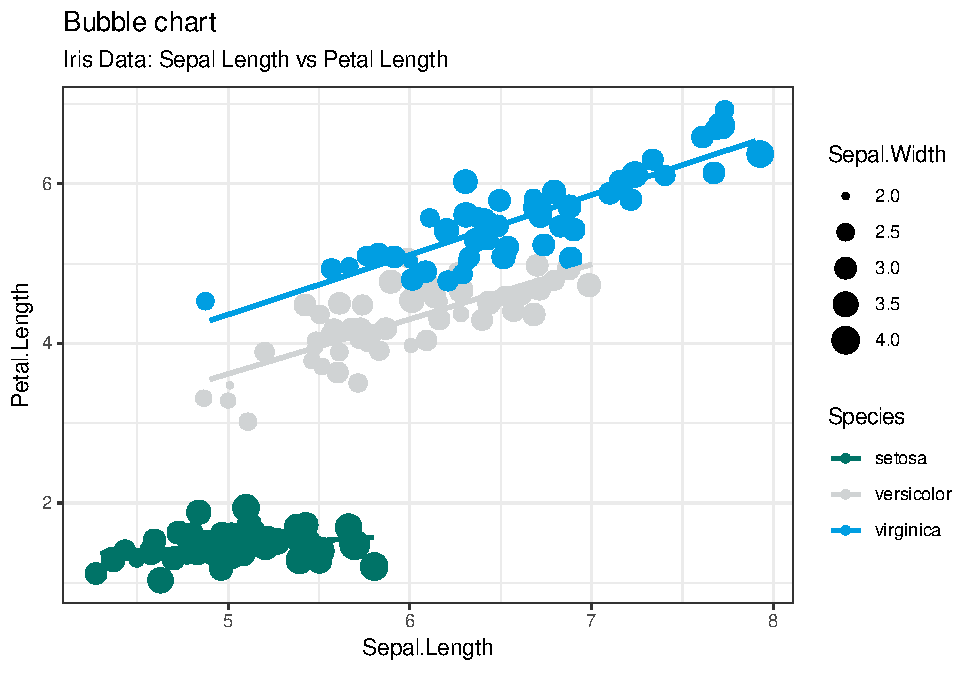
\includegraphics{figure/scatterPlot-1} \end{center}

\end{document}
